\documentclass[tikz,border=4pt]{standalone}
% Estilo común de los diagramas de bloques (se usa con \input en cada standalone)
\usepackage[defaultsans,scale=0.92]{lato}
\usepackage{libertinust1math}
\usepackage{xcolor,amsmath}
\usepackage{tikz}
\usetikzlibrary{positioning,arrows.meta,calc,shapes.geometric}
\usepackage{../../notacion}
\definecolor{ctrlazul}{HTML}{1E5AA8}\definecolor{ctrlnoche}{HTML}{14213D}
\definecolor{ctrlcoral}{HTML}{D1495B}\definecolor{ctrlverde}{HTML}{2A9D8F}
\definecolor{ctrlambar}{HTML}{E09F3E}\definecolor{ctrlgris}{HTML}{5C677D}
\definecolor{ctrlvioleta}{HTML}{6C4AB6}\definecolor{ctrlteal}{HTML}{0F7173}
\tikzset{
  >={Stealth[length=2.4mm]}, every node/.style={font=\small},
  bloque/.style={draw=ctrlnoche,fill=ctrlazul!7,thick,rounded corners=1.5pt,minimum height=9mm,minimum width=13mm,inner sep=4pt},
  suma/.style={draw=ctrlnoche,thick,circle,inner sep=0pt,minimum size=6mm},
  senal/.style={->,thick,draw=ctrlnoche},
  rot/.style={font=\footnotesize,text=ctrlgris},
}

\begin{document}
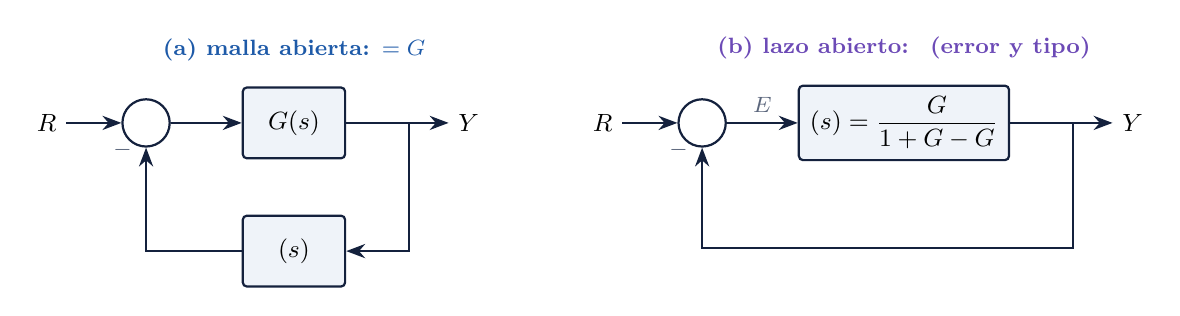
\begin{tikzpicture}[node distance=10mm]
  % (a) lazo general
  \node (ra) {$R$};
  \node[suma,right=7mm of ra] (Sa) {};
  \node[bloque,right=9mm of Sa] (Ga) {$G(s)$};
  \coordinate[right=8mm of Ga] (ya0); \node[right=5mm of ya0] (ya) {$Y$};
  \node[bloque,below=7mm of Ga] (Ha) {$\Hs(s)$};
  \draw[senal] (ra)--(Sa); \draw[senal] (Sa)--(Ga); \draw[senal] (Ga)--(ya);
  \draw[senal] (ya0) |- (Ha); \draw[senal] (Ha) -| (Sa); \node[rot] at ($(Sa)+(-3mm,-3.5mm)$) {$-$};
  \node[above=2mm of Ga,font=\footnotesize\bfseries,text=ctrlazul] {(a) malla abierta: $\Gma=G\Hs$};
  % (b) unitaria equivalente
  \node[right=12mm of ya] (rb) {$R$};
  \node[suma,right=7mm of rb] (Sb) {};
  \node[bloque,right=9mm of Sb,minimum width=24mm] (Gb) {$\Gla(s)=\dfrac{G}{1+G\Hs-G}$};
  \coordinate[right=8mm of Gb] (yb0); \node[right=5mm of yb0] (yb) {$Y$};
  \coordinate[below=11mm of Gb] (hb);
  \draw[senal] (rb)--(Sb); \draw[senal] (Sb)-- node[above,rot]{$E$} (Gb); \draw[senal] (Gb)--(yb);
  \draw[senal] (yb0) |- (hb) -| (Sb); \node[rot] at ($(Sb)+(-3mm,-3.5mm)$) {$-$};
  \node[above=2mm of Gb,font=\footnotesize\bfseries,text=ctrlvioleta] {(b) lazo abierto: $\Gla$ (error y tipo)};
\end{tikzpicture}
\end{document}
